%!TEX root = ../../book_ML.tex
\chapter{Ước lượng tham số mô hình}

 
 
 
\section{Giới thiệu}
% \textbf{Những sự kiện có xác suất cao là những sự kiện có khả năng xảy ra hơn.} 
 
% Câu nói \textit{nói cũng như không này} là khơi nguồn cho rất nhiều các thuật toán Machine Learning có liên quan đến xác suất. 
 
% Một mô hình machine learning thường bao gồm ba thành phần: 
% \textbf{Modeling, Learning} và \textbf{Inference}\footnote{Xem Chương 6 của
% \href{http://www.computervisionmodels.com/}{Computer Vision: Models, Learning,
% and Inference}}.
 
% \textbf{Modeling là việc đi tìm môt mô hình thích hợp cho bài toán cần giải
% quyết.} Với bài toán linear regression, modeling chính là việc mô hình dữ liệu
% đầu ra như là tổ hợp tuyến tính của các đặc trưng. Với bài toán k-means
% clustering, modeling chính là việc quan sát ra rằng các clusters thường được mô
% tả bởi các \textit{centroids} và mỗi điểm được xếp vào cluster tương ứng với
% centroid gần nó nhất. Việc đi tìm ra mô hình nào phù hợp cho bài toán chính là
% bước \textbf{modeling}.
 
% \textbf{Learning là bước tiến hành tối ưu các tham số của mô hình.} Với linear
% regression, tham số mô hình là bộ vector hệ số và bias $(\mathbf{w}, b)$. Quá
% trình tối thiểu hoá hàm mất mát của nó chính là
% quá trình đi tìm tham số của mô hình, chính là quá trình \textbf{learning}.
 
% \textbf{Inference là bước dự đoán đầu của mô hình khi có đầu vào mới.} Với
% linear regression, inference chính là việc tính $y = \mathbf{w}^T\mathbf{x} + b$
% dựa trên bộ các tham số đã được huấn luyện $(\mathbf{w}, b)$. So với hai bước
% modeling và learning, inference thường đơn giản hơn. 

% Với các mô hình xác Việc
% \textit{Inference} có thể coi
 
% Các mô hình machine learning thống kế (\textit{statistical machine learning})
% đóng vai trò 
\index{uoc@ước lượng tham số -- parameter estimation}
\index{tham số mô hình -- model parameter}
Có rất nhiều mô hình machine learning được xây dựng dựa trên các mô hình thống
kê. Các mô hình thống kê thường dựa trên các phân phối xác suất đã được đề cập
trong Chương~\ref{cha:prob}. Với một mô hình thông kê bất kỳ, ký hiệu $\theta$
là tập hợp tất cả các tham số của mô hình đó. Với phân phối Bernoulli, tham số
là biến $\lambda$. Với phân phối chuẩn nhiều chiều, các tham số là vector kỳ
vọng $\bmu$ và ma trận hiệp phương sai $\bSigma$.  ``Learning'' chính là quá
trình {ước lượng} bộ tham số $\theta$ sao cho mô hình tìm được khớp với phân
phối của dữ liệu nhất. Quá trình này còn được gọi là \textit{ước lượng tham số} (parameter estimation).

% \index{uoc@ước lượng hợp lý cực đại -- maximum likelihood estimation}
\index{uoc@ước lượng hậu nghiệm cực đại -- maximum a posteriori estimation}
\index{MAP estimation}

Có hai cách ước lượng tham số thường được dùng trong các mô hình machine
learning thống kê. Cách thứ nhất chỉ dựa trên dữ liệu đã biết trong tập huấn
luyện, được gọi là \textit{ước lượng hợp lý cực đại}({maximum likelihood
estimation} hay {ML estimation} hoặc \textit{MLE}). Cách thứ hai không
những dựa trên tập huấn luyện mà còn dựa trên những thông tin biết trước của các
tham số. Những thông tin này có thể có được bằng {cảm quan} của người xây dựng
mô hình. {Cảm quan} càng rõ ràng, càng hợp lý thì khả năng thu được bộ tham số
tốt càng cao. Chẳng hạn, thông tin biết trước của $\lambda$ trong phân phối
Bernoulli là việc nó là một số trong đoạn $[0, 1]$. Với bài toán tung đồng xu,
với $\lambda$ là xác suất có được mặt xấp, ta dự đoán được rằng giá trị này là
một số gần với $0.5$. Cách ước lượng tham số thứ hai này được gọi là \textit{ước
lượng hậu nghiệm cực đại} ({maximum a posteriori estimation} hay
{MAP estimation}). Trong chương này, chúng ta cùng tìm hiểu ý tưởng và
cách giải quyết bài toán ước lượng tham số mô hình theo {MLE} hoặc {MAP}.
 
 
\section{Ước lượng hợp lý cực đại}
\index{uoc@ước lượng hợp lý cực đại -- maximum likelihood estimation}
\index{MLE}
\subsection{Ý tưởng}
Giả sử có các điểm dữ liệu $\mathbf{x}_1, \mathbf{x}_2, \dots, \mathbf{x}_N$ tuân theo một phân phối nào đó được mô tả bởi bộ tham số $\theta$. 
 Ước lượng hợp lý cực đại là việc đi tìm bộ tham số $\theta$ để
\begin{equation} 
\label{eqn:31_1}
\theta = \argmax_{\theta} p(\mathbf{x}_1, \dots, \mathbf{x}_N | \theta).
\end{equation} 
Bài toán~\eqref{eqn:31_1} có ý nghĩa như thế nào và vì sao việc này hợp lý? 

\index{hàm hợp lý -- likelihood}
Giả sử rằng ta đã biết rằng mô hình có dạng đặc biệt được mô tả bởi bộ tham số
$\theta$. Xác suất có điều kiện $p(\mathbf{x}_1 | \theta)$ chính là xác suất xảy
ra {sự kiện} $\mathbf{x}_1$ trong trường hợp mô hình được mô tả bởi bộ tham số
$\theta$. Và $p(\mathbf{x}_1, \dots, \mathbf{x}_N | \theta)$ chính là xác suất
để toàn bộ các {sự kiện} $\mathbf{x}_1, \mathbf{x}_2, \dots, \mathbf{x}_N$ đồng
thời xảy ra, xác suất đồng thời này còn được gọi là \textit{sự hợp lý} ({likelihood}).

Phân phối của dữ liệu và bản thân dữ liệu có thể lần lượt được coi là nguyên nhân và kết quả. Ta cần tìm nguyên nhân (bộ tham số $\theta$) để khả năng xảy ra kết quả (hàm hợp lý) là cao nhất.

 
\subsection{Giả sử về sự độc lập và log-likelihood}
\index{log-likelihood}
Người ta thường ít khi giải trực tiếp bài toán~\eqref{eqn:31_1} vì khó tìm được
một mô hình xác suất đồng thời cho toàn bộ dữ liệu. Một cách tiếp cận phổ biến
khác là đơn giản hoá mô hình bằng cách giả sử các điểm dữ liệu $\mathbf{x}_n$
độc lập với nhau khi biết bộ tham số $\theta$. Nói cách khác, hàm hợp lý trong~\eqref{eqn:31_1} được xấp xỉ
bởi\footnote{Nhắc lại rằng nếu hai sự kiện $x, y$ là độc lập thì xác suất đồng thời bằng tích xác suất của từng sự kiện: $p(x, y) = p(x)p(y)$ và khi là
xác suất có điều kiện: $p(x, y | z) = p(x|z)p(y|z)$.}
\begin{equation} 
\label{eqn:31_2}
p(\mathbf{x}_1, \dots, \mathbf{x}_N | \theta) \approx \prod_{n = 1}^N p(\mathbf{x}_n |\theta).
\end{equation} 
 Lúc đó, bài toán~\eqref{eqn:31_1}
có thể được giải quyết bằng cách giải bài toán tối ưu 
\begin{equation} 
\label{eqn:31_3}
\theta = \argmax_{\theta} \prod_{n=1}^N p(\mathbf{x}_n| \theta) 
\end{equation} 
Mỗi giá trị $p(\bx_n |\theta)$ là một số dương nhỏ hơn một. Khi $N$ lớn, tích của các số dương này rất gần với 0, máy tính có thể không lưu chính xác được do sai số tính toán. Để tránh hiện tượng này, việc tối đa hàm mục tiêu thường được chuyển về việc tối đa logarit\footnote{Logarit là một hàm đồng biến.} của hàm mục tiêu:
\begin{equation} 
\label{eqn:31_4}
\theta = \argmax_{\theta} \log\left(\prod_{n=1}^N p(\mathbf{x}_n| \theta)\right) = \argmax_{\theta} \sum_{n = 1}^N \log\left(p(\mathbf{x}_n | \theta)
\right).
\end{equation} 

% \end{itemize}

% Chúng ta cùng xem vài ví dụ. 
 
 
\subsection{Ví dụ}
 
\subsubsection{Ví dụ 1: Phân phối Bernoulli}
\textbf{Bài toán}: Giả sử tung một đồng xu $N$ lần và nhận được $n$ mặt
ngửa, hãy ước lượng xác suất nhận được mặt ngửa khi tung đồng xu đó.
 
\textit{\textbf{Lời giải:}}

Một cách tự nhiên, ta có thể ước lượng được rằng xác suất đó chính là $\lambda
= \frac{n}{N}$. Chúng ta cùng ước lượng giá trị này bằng phương pháp MLE. 
 
Đặt $\lambda$ là xác suất để nhận được một mặt ngửa và $x_1, x_2,
\dots, x_N$ là các đầu ra quan sát thấy. Trong $N$ giá trị này, có $n$ giá trị bằng 1 tương ứng
với mặt ngửa và $m = N - n$ giá trị bằng 0 tương ứng với mặt
xấp. Nhận thấy 
\begin{equation} 
  \sum_{i=1}^N x_i = n, ~~N - \sum_{i=1}^N x_i = N - n = m.
\end{equation} 
Vì đây là một xác suất của biến ngẫu nhiên nhị phân rời rạc, sự kiện nhận được mặt ngửa hay xấp khi tung đồng xu tuân theo
phân phối Bernoulli:
\begin{equation} 
p(x_i | \lambda) = \lambda^{x_i} ( 1- \lambda)^{1 - x_i}.
\end{equation} 
Khi đó tham số mô hình $\lambda$ có thể được ước lượng bằng việc giải bài toán
tối ưu sau đây, với giả sử rằng kết quả của các lần tung đồng xu độc lập với
nhau:
% \begin{equation} 
\begin{alignat}{3}
  \lambda & =  \argmax_{\lambda}\left[ p(x_1, x_2, \dots, x_N | \lambda)\right] 
  % \label{eqn:31_5}
  && =  \argmax_{\lambda} \left[\prod_{i = 1}^N p(x_i | \lambda)\right] \\
  \label{eqn:31_6}
  & =  \argmax_{\lambda} \left[\prod_{i=1}^N  \lambda^{x_i} ( 1- \lambda)^{1 - x_i}\right]
  % \label{eqn:31_7}
  && = \argmax_{\lambda} \left[\lambda^{\sum_{i=1}^N x_i} (1 - \lambda)^{N - \sum_{i=1}^N x_i}\right]  \\\ 
  \label{eqn:31_8}
  & = \argmax_{\lambda} \left[\lambda^{n} (1 - \lambda)^{m}\right] 
  % \label{eqn:31_9}
  && = \argmax_{\lambda} \left[ n\log(\lambda) + m\log(1 - \lambda) \right] 
\end{alignat} 
% \end{equation} 
Tới đây, bài toán tối ưu~\eqref{eqn:31_8} có thể được giải bằng cách giải phương
trình đạo hàm của hàm mục tiêu bằng 0. Tức $\lambda$ là nghiệm của phương trình
\begin{eqnarray} 
  \frac{n}{\lambda} - \frac{m}{1 - \lambda}  =  0 
  \Leftrightarrow \frac{n}{\lambda}  =  \frac{m}{1 - \lambda} 
  \Leftrightarrow \lambda  =  \frac{n}{n + m} = \frac{n}{N} 
\end{eqnarray} 
% \end{equation} 
 
Vậy kết quả ước lượng ban đầu là có cơ sở. 
 
 
\subsubsection{Ví dụ 2: Phân phối categorical}
% Một ví dụ khác phức tạp hơn một chút. 

\textbf{Bài toán:} Giả sử tung một viên xúc xắc sáu mặt có xác suất rơi vào các
mặt không đều nhau. Giả sử trong $N$ lần tung, số lượng xuất hiện các mặt
thứ nhất, thứ hai,\dots, thứ sáu lần lượt là $n_1, n_2, \dots, n_6$ lần với
$\displaystyle \sum_{i=1}^6 n_i = N$. Tính xác suất rơi vào mỗi mặt. Giả sử thêm rằng $n_i > 0, ~\forall i = 1, \dots, 6.$
 
\lg 
 
Bài toán này phức tạp hơn bài toán trên, nhưng ta cũng có thể dự
đoán được ước lượng tốt nhất của xác suất rơi vào mặt thứ $i$ là $\lambda_i =
\frac{n_i}{N}$. 
 
{Mã hoá} mỗi kết quả đầu ra thứ $i$ bởi một vector 6 chiều $\mathbf{x}_i
\in \{0, 1\}^6$ trong đó các phần tử của nó bằng 0 trừ phần tử tương ứng với mặt
quan sát được bằng 1. Ta có  
  $\sum_{i=1}^N x^j_i = n_j, ~ \forall j = 1, 2, \dots, 6$,
trong đó $x^j_i$ là thành phần thứ $j$ của vector $\mathbf{x}_i$. 
 
Nhận thấy rằng xác suất rơi vào mỗi mặt tuân theo phân phối categorical với
các tham số $\lambda_j > 0, j = 1, 2, \dots, 6$. Ta dùng $\blambda$ để thể hiện
cho cả sáu tham số này. 

Với các tham số $\blambda$, xác suất để sự kiện $\mathbf{x}_i$ xảy ra là
\begin{eqnarray} 
  p(\mathbf{x}_i | \blambda) = \prod_{j = 1}^6 \lambda_j^{x_i^j} 
\end{eqnarray} 
% \end{equation} 
Khi đó, vẫn với giả sử về sự độc lập giữa các lần tung xúc xắc, ước lượng bộ
tham số $\lambda$ dựa trên việc tối đa log-likelihood ta có:
\begin{align} 
  % \lambda & = & \argmax_{\lambda} \left[ p(\mathbf{x}_1, \dots, \mathbf{x}_N  \| \lambda) \right]\\\ 
  \label{eqn:31_10}
  \blambda & =  \argmax_{\blambda} \left[ \prod_{i=1}^N p(\mathbf{x}_i |
  \blambda) \right] 
  % \label{eqn:31_11}
   =  \argmax_{\blambda} \left[ \prod_{i=1}^N  \prod_{j = 1}^6 \lambda_j^{x_i^j} \right]  \\\ 
  \label{eqn:31_12}
  & =  \argmax_{\blambda} \left[  \prod_{j = 1}^6 \lambda_j^{\sum_{i=1}^N x_i^j} \right] 
   =  \argmax_{\blambda} \left[  \prod_{j = 1}^6 \lambda_j^{n_j} \right]  \\\ 
  \label{eqn:31_14}
  & =  \argmax_{\blambda} \left[  \sum_{j=1}^6 n_j\log(\lambda_j) \right].
\end{align} 
% \end{equation} 
 Khác với bài toán~\eqref{eqn:31_8}, chúng ta không được quên điều kiện
$\sum_{j=1}^6 \lambda_j = 1$. Ta có bài toán tối ưu có ràng buộc sau đây:
\begin{equation}
\label{eqn:31_15}
\begin{aligned} 
  \max_{\lambda}  \sum_{j=1}^6 n_j\log(\lambda_j) \quad 
  \text{thoả mãn:}  \sum_{j=1}^6 \lambda_j = 1
\end{aligned} 
\end{equation}
Bài toán tối ưu này có thể được giải bằng phương pháp nhân tử Lagrange (xem Phụ
lục~\ref{apd:lagrange}).

Lagrangian của bài toán này là
\begin{equation} 
  \mathcal{L}(\lambda, \mu) = \sum_{j=1}^6 n_j\log(\lambda_j) + \mu (1- \sum_{j=1}^6 \lambda_j) 
\end{equation} 
Nghiệm của bài toán là nghiệm của hệ đạo hàm $\mathcal{L}(.)$ theo từng biến bằng 0:
\begin{alignat}{3}
\label{eqn:31_16}
\frac{\partial \mathcal{L}(\lambda, \mu)}{\partial \lambda_j} &=   \frac{n_j}{\lambda_j} - \mu &&=  0,~ \forall j = 1, 2, \dots, 6;\\
\label{eqn:31_17}
\frac{\partial \mathcal{L}(\lambda, \mu)}{\partial \mu} &=  1-\sum_{j=1}^6 \lambda_j &&= 0.
\end{alignat} 
Từ~\eqref{eqn:31_16} ta có $\lambda_j = \frac{n_j}{\mu}$. Thay
vào~\eqref{eqn:31_17}:
\begin{equation} 
  \sum_{j=1}^6 \frac{n_j}{\mu} = 1 \Rightarrow \mu = \sum_{j=1}^6 n_j = N 
\end{equation} 
Từ đó ta có ước lượng 
% \begin{equation} 
  $\lambda_j = \frac{n_j}{N}, ~~\forall j = 1, 2, \dots, 6$.
% \end{equation} 
 
Qua hai ví dụ trên ta thấy MLE cho kết quả khá hợp lý. 
 
 
\subsubsection{Ví dụ 3: Phân phối chuẩn một chiều}
 \label{sssec:gassian_mle}

\textbf{Bài toán:} Khi thực hiện một phép đo, giả sử rằng rất khó để có thể đo
{chính xác} độ dài của một vật. Thay vào đó, người ta thường đo vật đó
nhiều lần rồi suy ra kết quả, với giả thiết rằng các phép đo là độc lập với nhau
và kết quả mỗi phép đo là một phân phối chuẩn. Hãy ước lượng chiều dài của vật đó
dựa trên các kết quả đo được. 

\lg  
 Vì đã biết kết quả phép đo tuân theo phân phối chuẩn, ta sẽ đi tìm phân phối
chuẩn đó. Chiều dài của vật có thể được coi là giá trị mà hàm mật độ xác suất
đạt giá trị cao nhất. Trong phân phối chuẩn, ta biết rằng hàm mật độ xác suất
đạt giá trị lớn nhất tại kỳ vọng của phân phối đó. Chú ý rằng kỳ vọng của phân
phối và kỳ vọng của dữ liệu quan sát được có thể không bằng nhau, nhưng rất gần
nhau. Nếu ước lượng kỳ vọng của phân phối bằng MLE, ta sẽ thấy rằng kỳ vọng của
dữ liệu chính là đánh giá tốt nhất cho kỳ vọng của phân phối.
 
Thật vậy, giả sử các kích thước quan sát được là $x_1, x_2, \dots, x_N$. Ta cần
đi tìm một phân phối chuẩn, được mô tả bởi giá trị kỳ vọng $\mu$ và phương
sai $\sigma^2$, sao cho các giá trị $x_1, x_2, \dots, x_N$ là hợp lý nhất. Ta đã biết rằng, hàm mật độ xác suất tại $x_i$ của môt phân phối chuẩn có
kỳ vọng $\mu$ và phương sai $\sigma^2$ là
\begin{equation} 
  p(x_i | \mu, \sigma^2) = \frac{1}{\sqrt{2\pi \sigma^2}} \exp\left(-\frac{(x_i - \mu)^2}{2\sigma^2}\right).
\end{equation} 
Để đánh giá $\mu$ và $\sigma$, ta sử dụng MLE với giả thiết rằng kết quả
các phép đo là độc lập:
\begin{alignat}{3}
\label{eqn:31_18}
  \mu, \sigma & = 
  \argmax_{\mu, \sigma} \left[ \prod_{i=1}^N p(x_i | \mu,
  \sigma^2)\right]\\\ 
  \label{eqn:31_19}
  & =  \argmax_{\mu, \sigma} \left[ \frac{1}{(2\pi \sigma^2)^{N/2}} \exp\left(-\frac{\sum_{i=1}^N (x_i - \mu)^2}{2\sigma^2} \right) \right]\\\ 
  \label{eqn:31_20}
  & =  \argmax_{\mu, \sigma}\left[ -N\log(\sigma) - \frac{\sum_{i=1}^N (x_i - \mu)^2}{2\sigma^2} \triangleq J(\mu, \sigma) \right].
\end{alignat} 
Ta đã lấy logarit của hàm bên trong dấu ngoặc vuông của~\eqref{eqn:31_19} để
được~\eqref{eqn:31_20}, phần hằng số có chứa $2\pi$ cũng đã được bỏ đi vì
không ảnh hưởng tới kết quả.
 
Để tìm $\mu$ và $\sigma$, ta giải hệ phương trình đạo hàm của
$J(\mu, \sigma)$ theo mỗi biến bằng không: 
\begin{alignat}{3} 
\label{eqn:31_21}
  \frac{\partial J}{\partial \mu} & = \frac{1}{\sigma^2}\sum_{i=1}^N(x_i - \mu) = 0 \\
\label{eqn:31_22}
  \frac{\partial J}{\partial \sigma} & =  -\frac{N}{\sigma} + \frac{1}{\sigma^3}
  \sum_{i=1}^N (x_i - \mu)^2  = 0 \\
% \begin{equation} 
\imply 
  \mu  &=  \frac{\sum_{i=1}^N x_i}{N}, \quad 
  \sigma^2  =  \frac{\sum_{i=1}^N (x_i - \mu)^2}{N}.
% \end{equation} 
\end{alignat} 
 
Kết quả thu được không có gì bất ngờ.
 
 
\subsubsection{Ví dụ 4: Phân phối chuẩn nhiều chiều}
\textbf{Bài toán:} Giả sử tập dữ liệu ta thu được là các giá trị nhiều chiều
$\mathbf{x}_1, \dots, \mathbf{x}_N$ tuân theo phân phối chuẩn. Hãy đánh giá
vector kỳ vọng $\bmu$ và ma trận hiệp phương sai $\bSigma$ của phân phối này bằng MLE, giả sử rằng các $\mathbf{x}_1, \dots, \mathbf{x}_N$ độc lập.
 
\lg

Việc chứng minh các công thức
\begin{eqnarray} 
  \bmu & = & \frac{\sum_{i=1}^N \mathbf{x}_i}{N}, \\\ 
  \bSigma & = & \frac{1}{N}\sum_{i=1}^N (\mathbf{x} - \mu)(\mathbf{x} - \mu)^T 
\end{eqnarray} 
xin được dành lại cho bạn đọc như một bài tập nhỏ. Dưới đây là một vài gợi ý:

\begin{itemize}
    \item Hàm mật độ xác suất của phân phối chuẩn nhiều chiều là
    \begin{equation} 
      p(\mathbf{x} | \bmu, \bSigma) = \frac{1}{(2\pi)^{D/2} |\bSigma|^{1/2}} \exp \left(-\frac{1}{2} (\mathbf{x} - \bmu)^T \bSigma^{-1} (\mathbf{x} - \bmu)\right).
    \end{equation} 
    Chú ý rằng ma trận hiệp phương sai $\bSigma$ là xác định dương nên có nghịch đảo. 
    \item Một vài đạo hàm theo ma trận: 
    \begin{align} 
      \nabla_{\bSigma} \log |\bSigma| &= (\bSigma^{-1})^T \triangleq
      \bSigma^{-T}~~~ \text{(chuyển vị của nghịch đảo)}\\ 
      \nabla_{\bSigma} (\mathbf{x}_i - \bmu)^T \bSigma^{-1} (\mathbf{x}_i-\bmu) &= -\bSigma^{-T}(\mathbf{x}_i - \bmu)(\mathbf{x}_i - \bmu)^T\bSigma^{-T} 
    \end{align} 
\end{itemize}
(Xem thêm \textit{Matrix Calculus}, mục D.2.1 và D.2.4 tại
\url{https://goo.gl/JKg631}.) 
 
 
\section{Ước lượng hậu nghiệm cực đại}
\index{uoc@ước lượng hậu nghiệm cực đại -- maximum a posteriori estimation, MAP estimation}
\index{MAP}
\subsection{Ý tưởng}
Quay lại với Ví dụ 1 về bài toán tung đồng xu. Nếu tung đồng xu 5000 lần và nhận
được 1000 lần ngửa, ta có thể đánh giá xác suất nhận được mặt ngửa là $1/5$ và
việc đánh giá này là đáng tin vì số mẫu lớn. Nếu tung năm lần và chỉ nhận được
một mặt ngửa, theo MLE, xác suất để có một mặt ngửa được ước lượng là $1/5$. Tuy
nhiên với chỉ năm kết quả, ước lượng này là không đáng tin. Khi tập huấn luyện
quá nhỏ, ta cần quan tâm thêm tới một vài giả thiết của các tham số. Trong
ví dụ này, giả thiết của ta là xác suất nhận được mặt ngửa phải gần bằng $1/2$.
 
\textit{Ước lượng hậu nghiệm cực đại} (maximum a posteriori, MAP) ra
đời nhằm giải quyết vấn đề này. Trong MAP, ta giới thiệu một giả thiết biết
trước của tham số $\theta$. Từ giả thiết này, ta có thể
suy ra các khoảng giá trị và phân bố của tham số.
 
\index{xác suất hậu nghiệm -- posterior probability}
Khác với MLE, trong MAP, ta đánh giá tham số như một xác suất có
điều kiện của dữ liệu:
\begin{equation} 
\label{eqn:31_34}
  \theta = \argmax_{\theta} \underbrace{p(\theta | \mathbf{x}_1, \dots, \mathbf{x}_N)}_{\text{hậu nghiệm}}.
\end{equation} 
Biểu thức $p(\theta | \mathbf{x}_1, \dots, \mathbf{x}_N) $ còn được gọi là
{xác suất hậu nghiệm} của $\theta$. Chính vì vậy, việc ước lượng
$\theta$ theo~\eqref{eqn:31_34} được gọi là ước lượng hậu nghiệm cực đại.
 
Thông thường, hàm tối ưu trong~\eqref{eqn:31_34} khó xác định dạng một cách trực
tiếp. Chúng ta thường biết điều ngược lại, tức nếu biết tham số, ta có thể tính
được hàm mật độ xác suất của dữ liệu. Vì vậy, để giải bài toán MAP, quy tắc Bayes thường được sử dụng. Bài toán MAP được biến đổi thành
\begin{align} 
  \label{eqn:31_35}
  \theta & =  \argmax_{\theta} p(\theta | \mathbf{x}_1, \dots, \mathbf{x}_N) 
   =  \argmax_{\theta} \left[ \frac{\overbrace{p(\mathbf{x}_1, \dots,
  \mathbf{x}_N | \theta)}^{\text{hàm hợp lý}}
  \overbrace{p(\theta)}^{\text{tiên nghiệm}}}{p(\mathbf{x}_1, \dots, \mathbf{x}_N)} \right] \\ 
  \label{eqn:31_36}
  & =  \argmax_{\theta} \left[ p(\mathbf{x}_1, \dots, \mathbf{x}_N | \theta)
  p(\theta) \right] \\
  \label{eqn:31_37}
  & =  \argmax_{\theta} \left[ \prod_{i=1}^N p(\mathbf{x}_i | \theta) p(\theta) \right].
\end{align} 
 
Đẳng thức~\eqref{eqn:31_35} xảy ra theo quy tắc Bayes. Đẳng
thức~\eqref{eqn:31_36} xảy ra vì mẫu số của~\eqref{eqn:31_35} không phụ thuộc vào
tham số $\theta$. Đẳng thức~\eqref{eqn:31_37} xảy ra nếu có giả thiết về
sự độc lập giữa các $\mathbf{x}_i$. 

\index{tiên nghiệm -- prior}

Như vậy, điểm khác biệt lớn nhất giữa hai bài toán tối ưu MLE và MAP là việc hàm
mục tiêu của MAP có thêm $p(\theta)$, tức phân phối của $\theta$. Phân phối này
chính là những thông tin biết trước về $\theta$ và được gọi là
\textit{tiên nghiệm} (prior). Ta kết luận rằng hậu nghiệm tỉ lệ thuận với
tích của hàm hợp lý và tiên nghiệm.
 

Để chọn tiên nghiệm chúng ta cùng làm quen với một khái
niệm mới: \textit{tiên nghiệm liên hợp} (conjugate prior). 
 
 
\subsection{Tiên nghiệm liên hợp}
\index{tiên nghiệm liên hợp -- conjugate prior}
\index{phân phối liên hợp -- conjugate distribution}
Nếu phân phối hậu nghiệm $p(\theta | \mathbf{x}_1, \dots,
\mathbf{x}_N)$ có cùng dạng với phân phối tiên nghiệm $p(\theta)$, hai phân phối này được gọi là cặp \textit{phân phối liên hợp} (conjugate distribution), và $p(\theta)$ được
gọi là \textit{tiên nghiệm liên hợp} của hàm hợp lý $p(\mathbf{x}_1, \dots,
\mathbf{x}_N | \theta)$. Ta sẽ thấy rằng bài toán MAP và MLE có cấu trúc giống nhau. 
% Nếu \textit{posterior distribution} $p(\theta \| \mathbf{X})$ và \textit{likelihood} $p(\mathbf{X} \|\theta)$ có cùng \textit{họ} (family), thì \textit{prior distribution} là \textit{conjugate distribution} của \textit{likelihood distribution}. 
 
% Tôi sẽ không đi sâu vào phần này, bạn đọc có thể đọc thêm \href{https://en.wikipedia.org/wiki/Conjugate_prior}{Conjugate prior}. 

Một vài cặp phân phối liên hợp\footnote{Đọc thêm:
\textit{Conjugate prior -- Wikipedia} (\url{https://goo.gl/E2SHbD}).}:

\begin{itemize}
    \item Nếu hàm hợp lý và tiên nghiệm cho vector kỳ vọng là các phân phối
    chuẩn thì phân phối hậu nghiệm cũng là một phân phối chuẩn. Ta nói rằng phân
    phối chuẩn liên hợp với chính nó, hay còn gọi là \textit{tự liên hợp} (self-conjugate).
     
    \item Nếu hàm hợp lý là một phân phối chuẩn và tiên nghiệm
    cho phương sai là một {phân phối gamma}, phân phối hậu nghiệm cũng là một phân phối chuẩn. Ta nói rằng phân phối gamma là tiên nghiệm liên hợp cho phương sai của phân phối chuẩn. 
     
    \item Phân phối beta là liên hợp của phân phối Bernoulli.
     
    \item Phân phối Dirichlet là liên hợp của phân phối categorical.
 
\end{itemize}
 
\subsection{Siêu tham số}
Xét phân phối Bernoulli với hàm mật độ xác suất
\begin{equation} 
  p(x | \lambda) = \lambda^x ( 1 - \lambda)^{1 - x}
\end{equation} 
và liên hợp của nó, phân phối beta, có hàm phân mật độ xác suất
\begin{equation} 
  p(\lambda) = \frac{\Gamma(\alpha + \beta)}{\Gamma(\alpha) \Gamma(\beta)} \lambda^{\alpha - 1} ( 1 - \lambda) ^{\beta - 1}.
\end{equation} 
Bỏ qua thành phần hằng số chỉ mang mục đích chuẩn hoá, ta có thể nhận thấy rằng
phần còn lại của phân phối beta có cùng dạng với phân phối Bernoulli. Cụ thể,
nếu sử dụng phân phối beta làm tiên nghiệm cho tham số $\lambda$, và bỏ qua
phần thừa số hằng số, hậu nghiệm sẽ có dạng
\begin{eqnarray} 
\nonumber 
  p(\lambda | x) & \propto & p(x | \lambda) p(\lambda) \\\ 
  \label{eqn:31_38}
      & \propto & \lambda^{x + \alpha - 1}(1 - \lambda)^{1 - x + \beta - 1}
\end{eqnarray}  
Nhận thấy~\eqref{eqn:31_38} {vẫn có dạng của một phân phối
Bernoulli.} Vì vậy, phân phối beta là một tiên nghiệm liên hợp của phân phối Bernoulli.

\index{siêu tham số -- hyperparameter} 
Trong ví dụ này, tham số $\lambda$ phụ thuộc vào hai tham số khác là $\alpha$ và
$\beta$. Để tránh nhầm lẫn, hai tham số $(\alpha, \beta)$ được gọi là các
\textit{siêu tham số} (hyperparameter). 
 
Quay trở lại ví dụ về bài toán tung đồng xu $N$ lần có $n$ lần nhận được mặt
ngửa và $m = N - n$ lần nhận được mặt xấp. Nếu sử dụng MLE,
ta nhận được ước lượng $\lambda = n/M$. Nếu sử dụng MAP với tiên nghiệm là một
$\text{beta}[\alpha, \beta]$ thì kết quả sẽ thay đổi thế nào? 
 
Bài toán tối ưu MAP
\begin{eqnarray} 
\nonumber
  \lambda & = & \argmax_{\lambda} \left[p(x_1, \dots, x_N | \lambda) p(\lambda) \right] \\\ 
\nonumber
  & = & \argmax_{\lambda} \left[\left(\prod_{i=1}^N \lambda^{x_i} ( 1- \lambda)^{1 - x_i}\right) \lambda^{\alpha - 1} ( 1 - \lambda)^{\beta - 1} \right] \\\ 
\nonumber
  & = & \argmax_{\lambda} \left[ \lambda^{\sum_{i = 1}^N x_i + \alpha - 1} ( 1- \lambda)^{N - \sum_{i=1}^N x_i + \beta - 1} \right] \\\ 
  \label{eqn:31_39}
  & = & \argmax_{\lambda} \left[ \lambda^{n + \alpha - 1} ( 1- \lambda)^{m + \beta - 1} \right] 
\end{eqnarray} 
 Bài toán tối ưu~\eqref{eqn:31_39} chính là bài toán tối ưu~\eqref{eqn:31_38} với
tham số thay đổi một chút. Tương tự như~\eqref{eqn:31_38}, nghiệm
của~\eqref{eqn:31_39} là
\begin{equation} 
\label{eqn:31_40}
\lambda = \frac{n + \alpha - 1}{n + m + \alpha + \beta - 2}= \frac{n + \alpha - 1}{N + \alpha + \beta - 2}
\end{equation} 
Việc chọn tiên nghiệm phù hợp đã khiến cho việc tối ưu bài toán MAP được thuận
lợi.
 
 
Việc còn lại là chọn cặp siêu tham số $\alpha$ và $\beta$. 
 
Chúng ta cùng xem lại dạng của phân phối beta và thấy rằng khi $\alpha
= \beta > 1$, hàm mật độ xác suất của phân phối beta đối xứng qua điểm 0.5 và
đạt giá trị cao nhất tại 0.5. Xét Hình~\ref{fig:31_1}, ta thấy rằng khi
$\alpha =\beta > 1$, mật độ xác suất xung quanh điểm 0.5 nhận giá trị
cao, điều này chứng tỏ $\lambda$ có xu hướng gần 0.5.
 
Nếu chọn $\alpha = \beta = 1$, ta nhận được phân phối đều vì đồ thị hàm mật
độ xác suất là một đường thẳng. Lúc này, xác suất của $\lambda$ tại mọi vị trí
trong khoảng $[0, 1]$ là như nhau. Thực chất, nếu ta thay $\alpha = \beta = 1$
vào~\eqref{eqn:31_40} ta sẽ thu được $\lambda = n/N$, đây chính là ước lượng thu
được bằng MLE. MLE là một trường hợp đặc biệt của MAP khi prior là một phân phối
đều.
 
\begin{figure}[t]
    % caption on side     
    \floatbox[{\capbeside\thisfloatsetup{capbesideposition={right,top},capbesidewidth=6cm}}]{figure}[\FBwidth]
    {\caption{ Đồ thị hàm mật độ xác suất của phân phối beta khi $\alpha =
    \beta$ và nhận các giá trị khác nhau. Khi cả hai giá trị này lớn, xác suất
    để $\lambda$ gần 0.5 sẽ cao hơn. }
    \label{fig:31_1}}
    { % figure here
    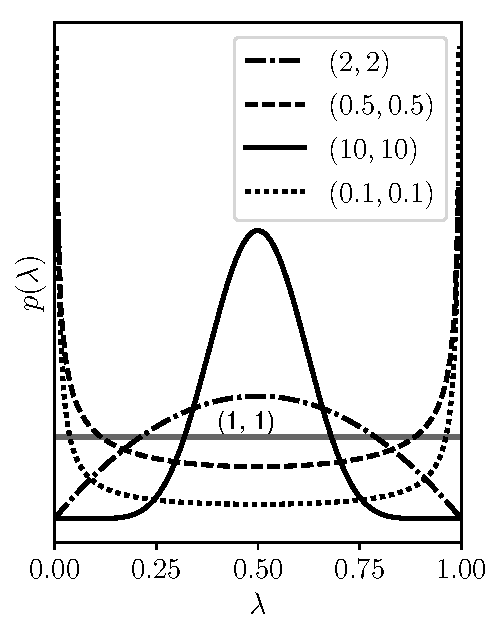
\includegraphics[width=.45\textwidth]{Chapters/02_LinearAlgebra/30_prob/python/beta1.pdf}
    }
\end{figure}

 
% <hr> 
% <div> 
% <table width = "100%" style = "border: 0px solid white"> 
%     <tr > 
%         <td height="100%" style = "border: 0px solid white" align = "center"> 
%         <img style="display:block;" width = "100%" src = "/assets/30_prob/beta1.png"> 
%          <br> 
 
%          </td> 
%          <td width="40%" style = "border: 0px solid white" align = "justify"> 
%          Hình 1: Đồ thị hàm mật độ xác suất của phân phối beta khi $\alpha = \beta$ và nhận các giá trị khác nhau. Khi cả hai giá trị này lớn, xác suất để $\lambda$ gần 0.5 sẽ cao hơn. 
%          </td> 
%     </tr> 
% </table> 
% </div> 
 
 
Nếu ta chọn $\alpha = \beta = 2$, ta sẽ thu được: 
\begin{math} \displaystyle 
  \lambda= \frac{n + 1}{N + 2} 
\end{math}.
Chẳng hạn khi $N = 5, n = 1$ như trong ví dụ. MLE cho kết quả $\lambda = 1/5$,
MAP sẽ cho kết quả $\lambda = 2/7$, gần với $1/2$ hơn. 
 
Nếu chọn $\alpha = \beta = 10$ ta sẽ có $\lambda = (1 + 9)/(5 + 18) = 10/23$. Ta
thấy rằng khi $\alpha = \beta$ và càng lớn thì ta sẽ thu được $\lambda$ càng gần
$1/2$. Điều này có thể dễ nhận thấy vì prior nhận giá trị rất cao tại 0.5 khi
các siêu tham số $\alpha = \beta$ lớn. 
 
 
% \subsection{MAP giúp tránh overfitting}
% Các siêu tham số thường được chọn dựa trên thực nghiệm, chẳng hạn bằng
% phương pháp hợp thức chéo. Việc thử nhiều bộ tham số rồi chọn ra bộ tốt nhất là việc mà
% các kỹ sư machine learning thường xuyên phải đối mặt. Cũng giống như việc chọn
% regularization parameter để tránh overfitting vậy.
 
% % Rõ ràng MAP cho chúng ta các kết quả \textit{linh hoạt} (flexible) với sự thay
% % đổi của hyperparameters. Và là một cách để tránh
% % \href{http://machinelearningcoban.com/2017/03/04/overfitting/}{overfitting}.
 
% Nếu viết lại bài toán MAP dưới dạng: 
% \begin{eqnarray} 
%   \theta & = & \argmax_{\theta} p(\mathbf{X}| \theta) p(\theta) \\\ 
%   & = & \argmax_{\lambda} \left[ \log \underbrace{p(\mathbf{X}| \theta)}_{\text{likelihood}} + \log \underbrace{p(\theta)}_{\text{prior}} \right] 
% \end{eqnarray} 
% ta có thể thấy rằng hàm mục tiêu có dạng $\L(\theta) + \lambda R(\theta)$ giống
% như trong regularization, với hàm log-likelihood đóng vai trò như hàm mất mát
% $\L(\theta)$, và log của prior đóng vai trò như hàm $R(\theta)$. Ta có thể nói
% rằng, MAP chính là một phương pháp giúp tránh overfitting trong các mô hình
% machine learning thống kê. MAP đặc biệt hữu ích khi tập huấn luyện là nhỏ. 

 
 
\section{Tóm tắt}
\begin{itemize}
    \item Khi sử dụng các mô hình thống kê machine learning, chúng ta thường
    xuyên phải ước lượng các tham số của mô hình $\theta$. Có hai phương pháp phổ biến được sử dụng để
    ước lượng $\theta$ là ước lượng hợp lý cực đại (MLE) và ước lượng hậu nghiệ cực đại (MAP).
     
    \item Với MLE, việc xác định tham số $\theta$ được thực hiện bằng cách đi
    tìm các tham số sao cho xác suất của tập huấn luyện, được xác định bằng
    hàm {hợp lý}, là lớn nhất: 
    \begin{equation} 
      \theta = \argmax_{\theta} p(\mathbf{x}_1, \dots, \mathbf{x}_N |\theta). 
    \end{equation} 
     
    \item Để giải bài toán tối ưu này, giả thiết các dữ liệu $\mathbf{x}_i$ độc lập thường được sử dụng. Và bài toán MLE trở thành
    \begin{equation} 
      \theta = \argmax_{\theta} \prod_{i=1}^N p(\mathbf{x}_i | \theta).
    \end{equation} 
     
    \item Với MAP, các tham số được đánh giá bằng cách tối đa {hậu nghiệm}: 
    \begin{equation} 
        \theta = \argmax_{\theta} p(\theta | \mathbf{x}_1, \dots, \mathbf{x}_N) 
    \end{equation} 
    \item Quy tắc Bayes và giả thiết về sự độc lập của dữ
    liệu thường được sử dụng: 
    \begin{equation} \theta = \argmax_{\theta}
        \left[\prod_{i=1}^N p(\mathbf{x}_i | \theta) p(\theta) \right]
    \end{equation} 
    Hàm mục tiêu ở đây chính là tích của {hàm hợp lý} và tiên nghiệm.

     
    \item Tiên nghiệm thường được chọn dựa trên các thông tin biết trước của
    tham số, và phân phối được chọn thường là các phân phối liên hợp của likelihood.
     
    \item MAP có thể được coi như một phương pháp giúp tránh thiên lệch khi có
    ít dữ liệu huấn luyện.
     
\end{itemize}
 
 
% \section{Đọc thêm}
% \begin{enumerate}
%     \item Chapter 4, 6 của \href{http://www.computervisionmodels.com}{Computer Vision:  Models, Learning, and Inference - Simon J.D. Prince.}
    
%     \item \href{https://en.wikipedia.org/wiki/Conjugate_prior}{Conjugate prior
%      --  Wikipedia.}

% \end{enumerate}
